%\subsection{Variación del contenido muónico}

Se hace hace necesario investigar el contenido muónico de la señal \textbf{Dark-}\SUSY~ bajo las diferentes condiciones de generación, para hacer referencia a estas condiciones iniciales con las que se generó la señal, se hará uso del vector:
\begin{equation}
\vec{\alpha} = (m_{n_1}, m_{n_D}, m_{\gamma_D}, c\tau_{\gamma_D})
\end{equation}
además el número de partículas $p$ en el i-ésimo evento generado está definido por:
\begin{equation}\label{numero_particulas}
n_i^{(p,k)} \equiv n_i^{(p,k)} (\vec{\alpha})
\end{equation}
donde 
$k =$ \begin{small}$\textsf{R2},~\textsf{HL}, ~\textsf{True}$\end{small}  declara la presencia del detector y su configuración, 
$i = 1, \ldots, N_{e}$ hace referencia al evento y 
$p = \mu^\pm, ~ \gamma_D, ~n_D, ~n_1$ a la partícula caracterizada.
%\begin{tabular}{lll}
%$k$ & $= \textsf{R2},~\textsf{HL}, ~\textsf{True}$ & declara la presencia del detector y su configuración.\\
%$i$ & $ = 1, \ldots, N_{e}$ & hace referencia al evento.\\
%$p$ & $ = \mu^\pm, ~ \gamma_D, ~n_D, ~n_1$ & partícula caracterizada.
%\end{tabular}
Definiendo a $f^{(p, k)}_\textsf{e} (x)\equiv f^{(p, k)}_\textsf{e} (x; \vec{\alpha})$ como la fracción del total de eventos poseedores de un número $x$ de partículas tipo $p$ de la señal generada bajo las condiciones iniciales $\vec{\alpha}$ y con la configuración del detector $k$ se tiene entonces:
%\mathbb{M} 
\begin{equation}\label{fe}
f^{(p, k)}_\textsf{e} (x)  = \dfrac{\sum\limits_{i=1}^{N_e} \delta_{x,n_i^{(p,k)}}}{\sum\limits_{i=1}^{N_e} \sum\limits_{x=0}^\infty \delta_{x,n_i^{(p,k)}}} = \dfrac{1}{N_e} \sum_{i=1}^{N_e} \delta_{x,n_i^{(p,k)}}
\end{equation}
donde $x\in\mathbb{N}$ pertenece al grupo de lo números naturales, $\delta_{x,n_i^{(p,k)}}$ es la función delta de Kronecker. %Por otro lado $\mathbb{F}^{(p, k)}_\textsf{e} (x)\equiv \mathbb{F}^{(p, k)}_\textsf{e} (x; \vec{\alpha})$ es la fracción del total de eventos que contienen muones de ruido no procedentes del decaimiento de la señal \MSSM\textbf{D}, dada por:
%\begin{equation}\label{fnInverso}
%\mathbb{F}^{(p, k)}_\textsf{e} (x)= 1 - f^{(p, k)}_\textsf{e}  (x; \vec{\alpha})
%\end{equation}
% ~~~ y ~~~ ff^{(p, k)}_\textsf{e} (\vec{\alpha}; x) = 1- f^{(p, k)}_\textsf{e} (\vec{\alpha}; x)
Finalmente, $f^{(p, k)}_\textsf{n} (x; \vec{\alpha}) \equiv f^{(p, k)}_\textsf{n} (x)$ es la fracción de partículas tipo $p$ que se encuentran en eventos con $x$ de estás partículas:
\begin{eqnarray}\label{fn}
f^{(p, k)}_\textsf{n} (x) & = \dfrac{\sum\limits_{i=1}^{N_e} n_i^{(p,k)} \delta_{x,n_i^{(p,k)}}}{\sum\limits_{i=1}^{N_e} \sum\limits_{n=0}^\infty n_i^{(p,k)} \delta_{n, n_i^{(p,k)}}}  = \dfrac{\sum\limits_{i=1}^{N_e} n_i^{(p,k)} \delta_{x, n_i^{(p,k)}}}{\sum\limits_{i=1}^{N_e} n_i^{(p,k)}}
\end{eqnarray}

%\begin{equation}
%\Delta f^{(\geqslant 4\mu, \backsim)}_\textsf{rel} = \left[ \sum_{i,n} \mathbb{E}_i^{(n\mu, \backsim)} - \sum_i \mathbb{E}_i^{(4\mu, \backsim)} \right]/\sum_{i,n} \mathbb{E}_i^{(n\mu, \backsim)}
%\end{equation}
%\begin{equation}
%\Delta f^{(\geqslant 4\mu, \backsim)}_\textsf{n} = \left[ \sum_{i,n} n \cdot \mathbb{E}_i^{(n\mu, \backsim)}- \sum_i 4 \cdot \mathbb{E}_i^{(4\mu, \backsim)}\right]/\sum_{i,n} n \cdot \mathbb{E}_i^{(4\mu, \backsim)}
%\end{equation}
%\begin{equation}
%\Delta f^{(\geqslant 4\mu, \textsf{True})}_\textsf{n} = \left[ \sum_{i} n^{(\mu,\textsf{True})}_i \cdot \mathbb{E}_i^{(\textsf{True})} \cdot (1- \textsf{IO}(n^{(\mu,\textsf{True})}_i,~ 4) \right]/\sum_{i} n^{(\mu,\textsf{True})}_i \cdot \mathbb{E}_i^{(\textsf{True})} 
%\end{equation}

Algunos ejemplos del contenido muónico de los eventos se muestran en la Fig. \ref{contenido_muonico}, donde se pueden visualizar los cambios con la masa del fotón oscuro $m_{\gamma_D}$ y la masa del neutralino oscuro $m_{n_D}$. La caracterización solo se realiza para $m_{n_1}=10$ GeV. Del conjunto de muestras simuladas con \MC ~ sin la reconstrucción del detector ($k=\textsf{True}$), se constató la invarianza de la distribución del contenido muónico $f^{(\mu, \textsf{True})}_\textsf{n} (x; \vec{\alpha}) $ ante los cambios de los parámetros de generación $\vec{\alpha}$, cuestión esperada por la teoría, ya que los muones de procesos de ruido son elementos que no se esperan estar relacionados con el proceso \textbf{Dark-}\SUSY ~ determinado por el decaimiento de la Fig. \ref{fig:sketch_darksector}b.

\begin{figure}[!ht]
\centering
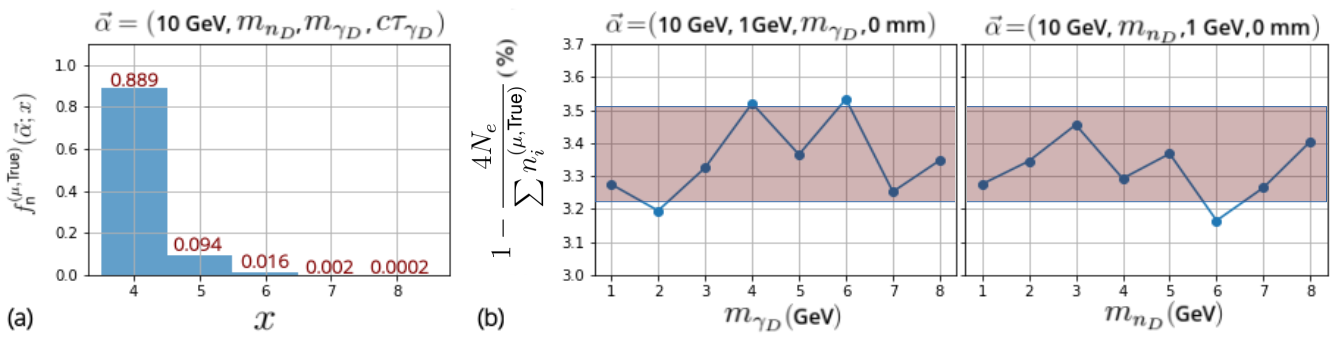
\includegraphics[width=1\textwidth]{Cap4/imagenes/True_Entries.png}
\caption{(a) Variación del contenido muónico de los eventos antes de pasar por el detector; (b) Variación del porciento de la fracción de muones de ruido con los parámetros de generación $m_{\gamma_D}$ y $M_{n_1}$.}
\label{contenido_muonico}
\end{figure}

De la Fig. \ref{contenido_muonico}a se conoce que el contenido mínimo de muones por evento para $k=\textsf{True}$ es de 4 muones, estos son el resultado de la recreación de la señal \MC ~ proveniente de \textbf{Dark-}\SUSY~ relacionada con el decaimiento de la Fig. \ref{fig:sketch_darksector}b. Los valores de $f^{(\mu, \textsf{True})}_\textsf{n} (x; \vec{\alpha}) $ con sus respectivos errores se pueden ver en la Tabla \ref{generacion0}, además, se hace supuesto de la caracterización de las Figs. \ref{contenido_muonico}b, que la fracción de los muones provenientes de señales de ruido se presenta alrededor de un valor constante, el mismo está dado por:
\begin{equation}
1- \frac{4 N_e}{\sum n_i^{(\mu, \textsf{True})}} = 0.0337 \pm 0.0014
\end{equation}


% \multicolumn{4}{cccccc}{Parámetros de generación ($\vec{\alpha}$)}
\begin{table}[!h]
\scriptsize
\centering
\begin{tabular}{|c|ccccc|}
\toprule
Variable & $x = 4$ & $x = 5$ & $x = 6$ & $x = 7$ & $x = 8$\\
\midrule
$f^{(\mu, \textsf{True})}_\textsf{n} (x)$ & 
$0.8892 \pm 0.0086$ & $0.0942 \pm  0.0090$ & $0.0161 \pm 0.0016$ & $0.0022 \pm 0.0006$ & $0.0002 \pm 0.0002$ \\
\bottomrule 
\end{tabular}%}
\caption{Fracción de eventos dependiente del contenido muónico. % para un arbitrario parámetro de generación $\vec{\alpha}$.
}
\label{generacion0}
\end{table}

Al analizar los resultados obtenidos, se pudo concluir, que el ruido muónico en la reconstrucción de la señal \MSSM\textbf{D} se encuentra en una fracción del total de eventos dada por $1 - f^{(\mu, \textsf{True})}_\textsf{n} (4; \vec{\alpha}) =  0.113 \pm 0.004 $, fracción no despreciable de nuestro conjunto. Los datos que se poseen no son adecuados para estudiar. Todos los resultados obtenidos  la correspondencia con la masa del neutralino ligero $m_{n_1}$, de aquí que las conclusiones dadas en la sección no la incluyen.

\subsection{Variación de las propiedades de los muones}

Analizar la señal \textbf{Dark}-\SUSY ~o \MSSM\textbf{D}~ mediante las propiedades de los muones sin la reconstrucción del detector dará una base de comparación y un mayor entendimiento de la teoría. Además, separar la información según los muones que provienen del decaimiento $h \rightarrow 2n_1 \rightarrow 2n_D + 2\gamma_D \rightarrow 2n_D + 4\mu$ del resto de los procesos se hace necesario para una mejor interpretación de la reconstrucción conjunta de las señales. Se introduce la notación de las propiedades de una partícula $p= n_1, ~n_D, ~\gamma_D, ~\mu$, siendo la distribución de frecuencia dada por:
\begin{equation}\label{Wpk}
\textsf{W}^{(p,k)} (\textsf{x}_j) \equiv \textsf{W}^{(p,k)} (\chi; \vec{\alpha}) ~~~~~~ \longrightarrow ~~~~~~ \textsf{W}^{(p,k)}_N (\textsf{x}_j) = \dfrac{\textsf{W}^{(p,k)} (\textsf{x}_j)}{ \sum\limits_{\textsf{x}_j} \textsf{W}^{(p,k)} (\textsf{x}_j)}
\end{equation}
donde $\textsf{x}_j$ hace referencia a la propiedad de interés, estás se pueden ver en la Tabla \ref{propiedades}.

\begin{figure}[!t]
\centering
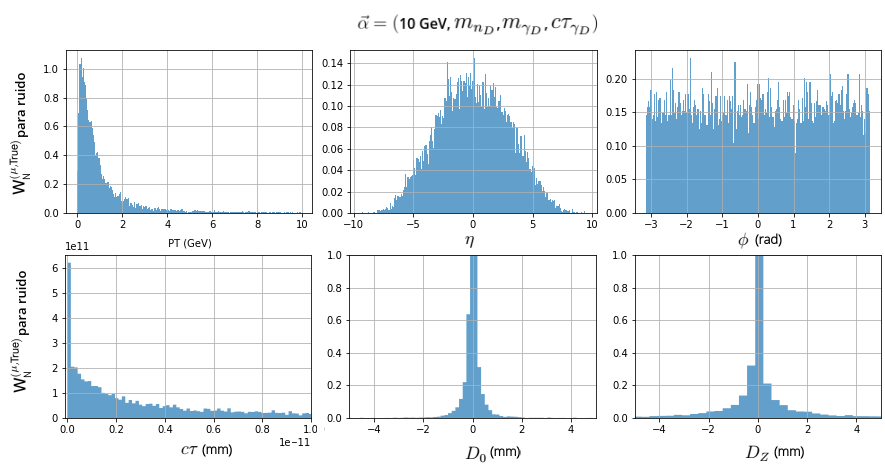
\includegraphics[width=.9\textwidth]{Cap4/imagenes/propiedades_True_notMSSM.png}
\caption{Variación de las distribuciones de los muones de procesos de ruido.}
\label{mu_True}

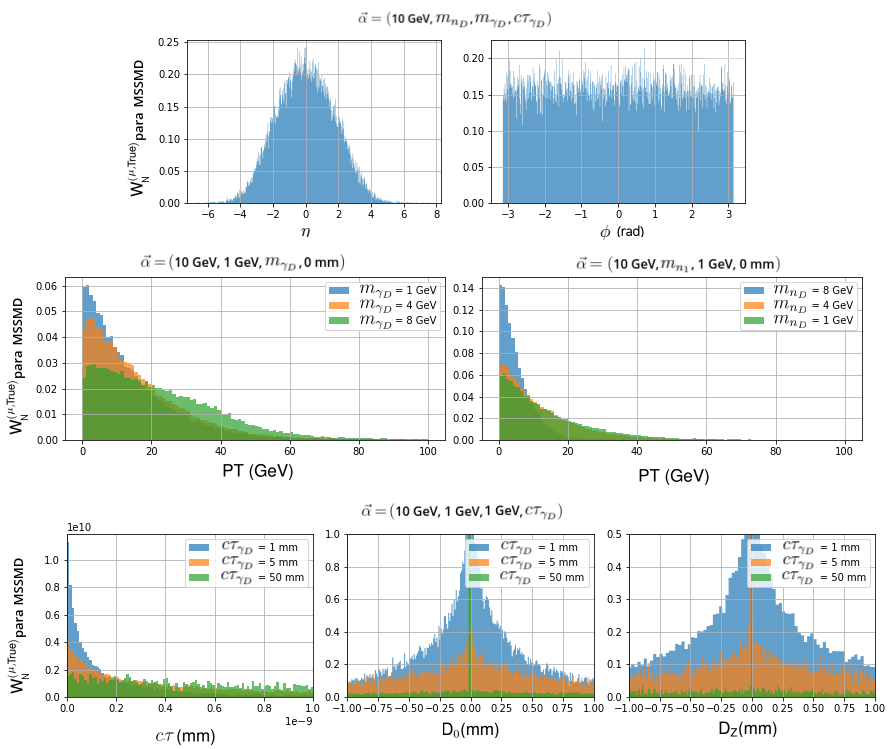
\includegraphics[width=.9\textwidth]{Cap4/imagenes/propiedades_True_MSSM.png}
\caption{Variación de las distribuciones de los muones caracteristicos de la señal \MSSM\textbf{D}.}
\label{mu_True2}
\end{figure}

Las distribuciones correspondientes a las propiedades de los muones $\textsf{W}^{(\mu,\textsf{True})}_N (\textsf{x}_j)$ proveniente de procesos alternos al decaimiento  \MSSM\textbf{D} se consideran ruido en esta investigación, sus propiedades se pueden visualizar en la Fig. \ref{mu_True}. Como resultado de su caraterización, se concluyó que la morfología de las distribuciones de ruido se mantiene con la variación de los parámetros de generación $\vec{\alpha}$. Además, el dominio para los valores del momento tranversal se extiende hasta $P_T= [0, 80]~ \textsf{GeV}$, pero el 98\% de los datos se agrupan para valores $<10~\textsf{GeV}$ como se visualiza en su respectiva distribución de la Fig. \ref{mu_True}.



Las distribuciones de las propiedades de los muones $\textsf{W}^{(\mu,\textsf{True})}_N (P_T)$ proveniente del decaimiento  \textbf{Dark-}\SUSY ~ (\MSSM\textbf{D}) se pueden visualizar en la Fig. \ref{mu_True2}. Con la comparación de las distribuciones con la variación de los elementos del parámetro de generación $\vec{\alpha}$, se comprobó la invarianza de la morfología de las distribuciones para los parámetros $\eta$ y $\phi$. Las distribuciones del momento transversal muestran variaciones con el parámetro de generación masa del fotón oscuro $m_{\gamma_D}$ y del neutralino oscuro $m_{n_D}$. Se concluye al comparar con las eficiencias de los detectores $k=\textsf{R2}, \textsf{HL}$ mostradas en las Figs. \ref{Compara_track_muon}, \ref{Compara_sol_muon} y \ref{Compara_eficiencia_muon}, que el aumento de la masa teórica del fotón oscuro permite un aumento de la probabilidad de detección de los muones que decaen de ellos, por el contrario el aumento teórico de la masa del neutralino oscuro dificultará la detección de muones de \MSSM\textbf{D} ya que estos estadisticamente tenderán a menores valores del momento. Los datos que se poseen no son adecuados para estudiar la correspondencia con la masa del neutralino ligero $m_{n_1}$, de aquí que las conclusiones dadas en la sección no la incluyen.


%Las distribuciones muestran que el $\sim 95$\% de los muones correspondientes al decaimiento \MSSM\textbf{D} ~ muestran su dominio para valores $PT < 80 \textsf{ GeV}$, para los muones resultantes de procesos de ruido tenemos $PT < 10 \textsf{ GeV}$. Además, se confirma una relación directa entre los estadísticos medios del momento transversal de los muones con el parámetro de generación masa del fotón oscuro $m_{\gamma_D}$, de forma inversa con el parámetro de masa del neutralino oscuro $m_{n_D}$.


\subsection{Características del fotón oscuro}
\begin{figure}[!h]
\centering
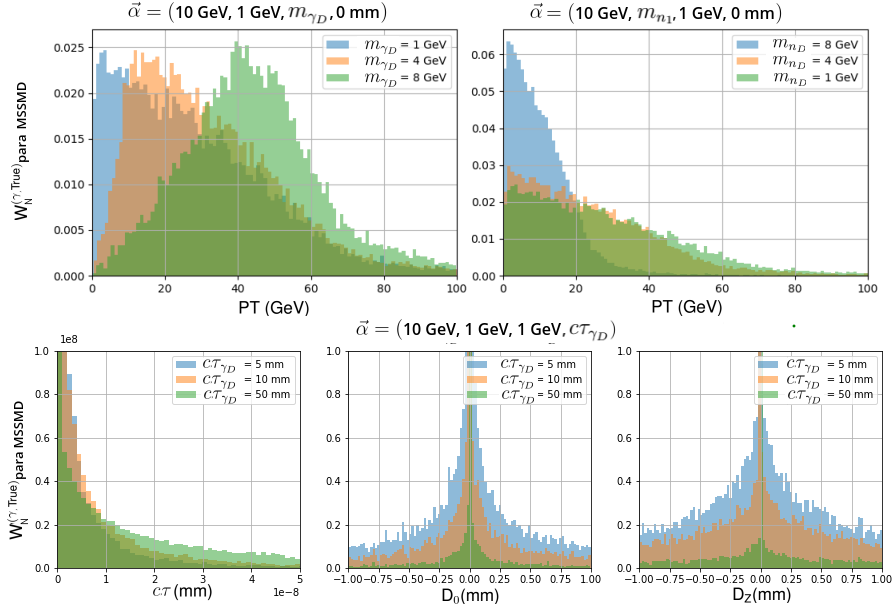
\includegraphics[width=.9\textwidth]{Cap4/imagenes/True_PT5.png}
\caption{Variación de las propiedades del fotón oscuro $\gamma_D$ con los parámetros de generación $m_{\gamma_D}$, $m_{n_D}$ y $\tau c_{\gamma_D}$.}
\label{PT_mu_True2}
\end{figure}
La reconstrucción del fotón oscuro $\gamma_D$ predicho por el decaimiento \MSSM\textbf{D} es el motivo principal de estudio de esta investigación. La caracterización de sus propiedades y el cambio de la morfología de los gráficos de frecuencias $\textsf{W}^{(\gamma , \textsf{True})}_N (\textsf{x}_j)$ con el cambio de los parámetros de generación $\vec{\alpha}$, permitirá una comprensión mas completa de los resultados obtenidos con la reconstrucción realizada por los detectores en la configuración Run-2 ($\textsf{R2}$) y Alta Luminosidad ($\textsf{HL}$).




Los gráficos de la Fig. \ref{PT_mu_True2} muestra la clara dependencia del momento angular $P_T$ y con los parámetros de masa de $\vec{\alpha}$, ya que son la masa del fotón $m_{\gamma_D}$ y su tiempo de vida $c\tau_{\gamma_D}$ son tratados por la teoría como parámetros libres, no hay dependencia directa entre ellas. Hay una correspondencia clara entre los parámetros de impacto $D_\textsf{0}$ y $D_\textsf{Z}$ como se esperaría con el parámetro de generación $c\tau_{\gamma_D}$.







